\section{Related Work}
Multi-GPUs are widely used for scaling single GPU perfromance
via integration of multiple GPUs at the system
level~\cite{pascal-tesla-wp,dgx,intersect360,titan_supercomputer} for a
rapidly growing pool of applications~\cite{coral,cudnn,Lavin15b,SimonyanZ14a}.
Similarly, multi-socket and multi-node CPU
installations have been employed and studied in context of HPC and
data-center applications~\cite{Intel:Xeon,IBM:Power,IBM:z196,AMD:Opteron}

Multi-GPU programming models require explicit programming of multiple GPUs
using SW APIs such as Peer-2-Peer access~\cite{NVIDIAP2P} or a combination of
MPI and CUDA~\cite{NVIDIAMPI} to manage multiple GPUs. These extensions require
unique programming experience and non-negligible SW effort while adapting a
single GPU application to take advantage of a Multi-GPU system. In this paper
we execute single GPU application on a Multi-GPU system as if it was a single
larger GPU via hardware innovations and extensions to the driver software to
provide programmer- and OS-transparent execution, similarly to approaches
proposed in the past~\cite{Cabezas2015,lee2013transparent,ben2015memory}.

Modern multi-socket CPU and GPU systems leverage most advanced interconnect
technologies such as Nvidia Nvlink, Intel QPI and AMD
Infinity~\cite{dgx,INTELQPI,AMDINFINITYFABRIC}. These modern fabrics utilize
high speed serial signalling technologies over unidirectional lanes
collectively comprizing full-duplex links. This way each link capacity is
statically allocated at design time and usually is symmetric in nature. In this
paper we propose to dynamically re-allocate available link bandwidth resources
by using same system wire resources and on-chip I/O interfaces, while
implementing both recever and transmitter driver circuitry at each lane. This
approach resembles previously proposed tri-state bi-directional bus
technologies ~\cite{tri-state}, or former technologies such as Intel front-side
bus ~\cite{fsb}. Our proposal however allows leveraging fast
singled ended signalling, while allowing a dynamically controlled
asymmetric bandwidth allocation via on-the-fly reconfiguration of the
individual lane direction within a link.

Static and dynamic cache partitioning techniques were widely explored in
context of CPU caches and QoS
~\cite{ics2007,Herdrich2016CacheQF,pact06,qureshi-micro,jaleel-pact} For
example, Rafique et al~\cite{pact06} proposed architectural support for shared
cache management with quota-based approach. Qureshi et al~\cite{qureshi-micro}
proposed to partition the cache space between applications. Jaleel et
al~\cite{jaleel-pact} improved on this by proposing adaptive insertion
policies. Recently, cache monitoring and allocation technologies were added to
Intel Xeon procesors, targeted for QoS enforcement via dynamic repartitioning
of on-chip CPU cache resources~\cite{Herdrich2016CacheQF}.  Efficient cache
partitioning in GPU was primarly explored in context of L1 caches
~\cite{li-priority-based}. While dynamic cache paritioning was widely used for
QoS and L1 utlization, to the best of our knowledge it was never used for
\ldots

% While MCMs are popular
%in various domains, we are unaware of any attempt to integrate
%homogeneous high performance GPU modules on the same package in an OS
%and programmer transparent fashion. To the best of our knowledge, this
%is the first effort to utilize MCM technology to scale GPU
%performance.


%The MCM-GPU design exposes a non-uniform memory accesses (NUMA)
%architecture. One of the main mechanisms to improve performance of
%NUMA systems is to preserve locality by assigning threads in close
%proximity to the data. In a multi-core domain, existing work tries to
%minimize the memory access latency by thread-to-core
%mapping~\cite{tam2007thread,blagodurov2010case,li1993locality}, or
%memory allocation
%policy~\cite{bolosky1989simple,larowe1991exploiting,dashti2013traffic}.
%Similar problem exists in MCM-GPU systems where the primary bottleneck
%is inter-GPM interconnection bandwidth. Moreover, improved CTA
%scheduling has been proposed to exploit the inter-CTA locality, higher
%cache hit ratios, and memory bank-level
%parallelism~\cite{leehpca2014,mao2016temp,wanglaperm} for monolithic
%GPUs. In our case, distributed CTA scheduling along with first-touch
%memory mapping policy exploits inter-CTA localities both within a
%kernel and across multiple kernels and improves efficiency of newly
%introduced GPM-side L1.5 cache.

%Finally, we propose to expose MCM-GPU as a single GPU via hardware
%innovations and extensions to the driver software to provide
%programmer- and OS-transparent execution. The runtime divides a
%given kernel into multiple sub-kernels and dispatches them to the CTA
%scheduler on each GPM, providing first-touch page allocation policy.
%Similarly, there have been studies on efficiently utilizing multi-GPU
%systems~\cite{Kim2011,Cabezas2015,lee2013transparent,ben2015memory},
%but none of the proposals provided a fully transparent approach
%suitable for MCM-GPUs.

% 
% % 
% % One use case in the future
% % may be that GPU programmers will size their application's data to extend well 
% beyond
% % the performance-optimal footprint in CPU and GPU memory.  With excess data 
% spilling over
% % into the additional capacity provided by the CPU memory, performance
% % bottlenecks will shift away from the GPU towards the CPU memory system.  In 
% such
% % cases, the GPU caching policy for CPU memory will come under additional 
% pressure due to
% % the increased traffic skewed towards CPU memory.
% % 
% % To understand how selective caching affects performance under such a scenario, 
% we evaluate
% % a situation wherein the application data has been
% % sized so that 90\% of the footprint resides in CPU memory and just 10\% can 
% fit within GPU memory, as compared to the nearly
% % inverse performance-optimal 20\%-80\% ratio.
% % Figure~\ref{fig:capacityconstrained} shows the performance of this 
% memory-capacity-constrained case relative 
% % to the baseline optimal ratio.  We see that naive selective caching and
% % our proposed enhancements follow the same trend of performance improvements
% % shown previously in Section~\ref{results}.  Because this scenario is primarily 
% limited
% % by the CPU memory system, we see that in some cases the client cache and 
% variable sized transfer interconnect optimizations
% % can actually outperform the hardware cache-coherent GPU due to a reduction in 
% data overfetch between the CPU memory and the GPU client.
% % To validate our observation, we added the same client cache and variable
% % transfers to the hardware cache-coherent baseline configuration and saw an 
% average
% % speedup of 4.5\%.  Whereas the absolute
% % performance achieved, compared to a performance-optimal memory footprint and 
% allocation, may not always be compelling, should
% % software designers chose to partition their problems in this way, we believe 
% selective caching will continue to 
% % perform as well as a hardware cache-coherent GPU.
% % 
% % \begin{figure}[t]
% % 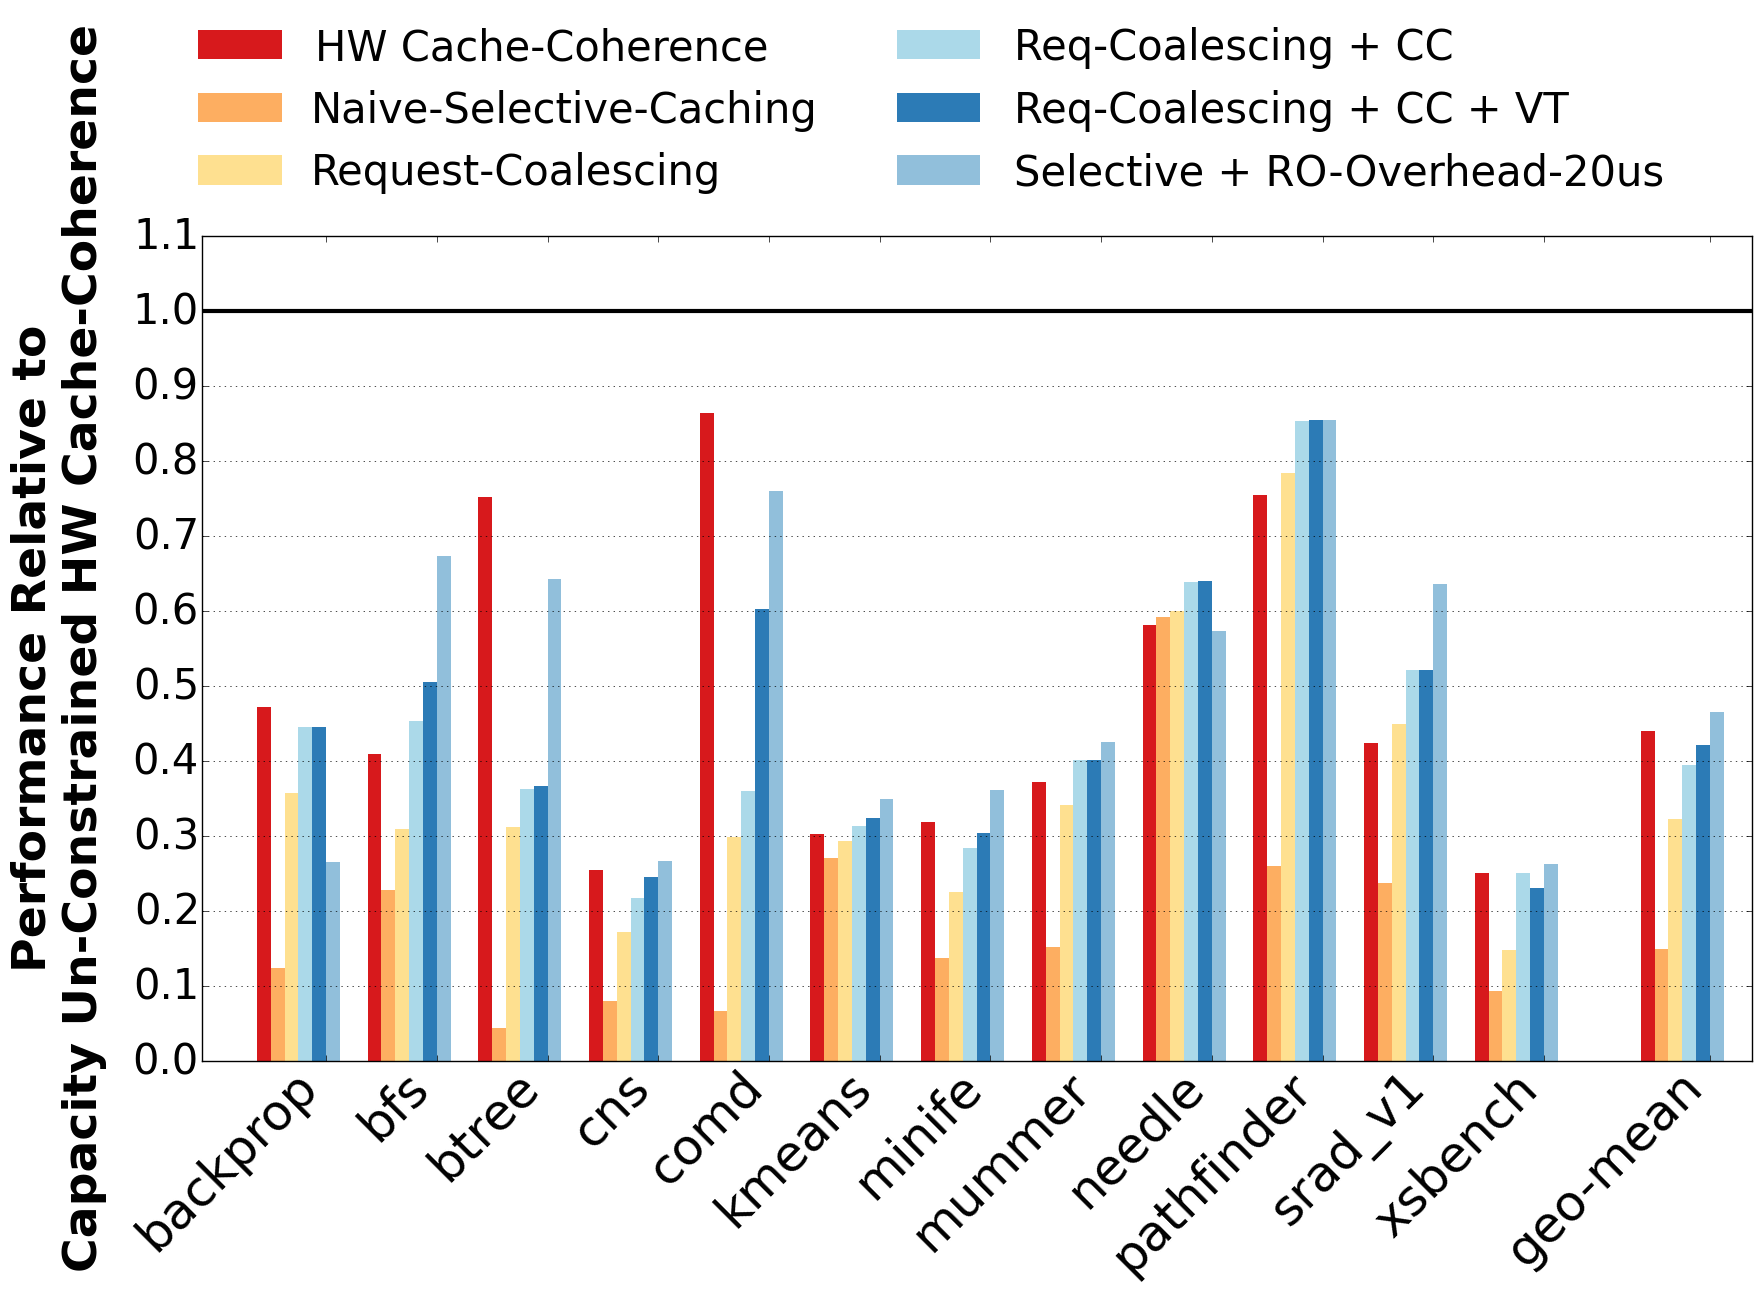
\includegraphics[width=1.0\columnwidth]{figures/capacityconstrained.png}
% % \caption{GPU performance under memory capacity constraints. (CC: Client-Cache,
% % VT: Variable-sized Transfer Units)}
% % \label{fig:capacityconstrained}
% % \end{figure}
% % 
% % In this work, we have primarily investigated a system where bandwidth-aware 
% page placement
% % provides an initial page placement that has been shown to have optimal 
% performance~\cite{Agarwal2015}.
% % Bandwidth-aware page placement is based on the premise that the GPU will place 
% pressure on
% % the CPU and GPU memory system in proportion to the number of pages placed in 
% each memory.  Proposals
% % like selective caching that change the on-chip caching policy of the GPU can 
% cause dramatic
% % shifts in the relative pressure placed on each memory system, effectively 
% changing the bandwidth-optimal 
% % placement ratio.  Although we do not evaluate this phenomenon in this work, 
% balancing
% % initial page placement with dynamic page migration to help compensate for the 
% lack of on-chip
% % caching is an area that needs further investigation.
% % 
% % \section{Related Work}
% % \label{related_work}
% % 
% % Cache coherence for CPUs has received great attention in the literature.
% % Recent proposals have started to explore intra-GPU and CPU--GPU cache 
% coherence.
% % 
% % \textbf{CPU Systems:} Scalable cache coherence has been studied extensively 
% for CPU-based
% %  multicore systems. Kelm et al. show that scaling up coherence to hundreds
% % or thousands of cores will be difficult without moving away from pure
% % hardware-based coherence~\cite{Kelm2009,Hill92}, due to high directory storage
% % overheads and coherence traffic~\cite{Lebeck95,Cheng06}.  
% % Whereas some groups have
% % evaluated software shared memory implementations~\cite{Falsafi94,Hill92}, 
% Martin
% % et al. argue that hardware cache coherence for mainstream processors is here 
% to
% % stay, because shifting away from it simply shifts the burden of correctness 
% into
% % software instead of hardware~\cite{Martin2012}. Nevertheless, disciplined 
% programming
% % models coupled with efficient hardware implementations are still being 
% pursued~\cite{choi2011,Sung2013,Sung2015}.
% % 
% % Self-invalidation protocols have been proposed to reduce invalidation traffic 
% and reduce
% % coherence miss latency~\cite{Lebeck95,Lai2000}. Our selective caching request 
% coalescing scheme uses a similar idea,
% % discarding a block immediately after fulfilling requests pending at the MSHR.
% % Other proposals have classified data into private, shared, and
% % instruction pages and have devised techniques to curtail coherence 
% transactions
% % for private data~\cite{Pugsley2010,Hardavellas2009,Cuesta2011,Ros2012}. We 
% instead classify
% % pages into read-only versus read-write and exploit the fact that read-only 
% data
% % can be safely cached in incoherent caches.
% % 
% % Ros and Kaxiras~\cite{Ros2012} have proposed a
% % directory\hyp{}less\slash{}broadcast\hyp{}less coherence protocol where all 
% shared
% % data is self\hyp{}invalidated at synchronization points. In this scheme,
% % at each synchronization point (e.g., lock acquire/release, memory barrier) all
% % caches need to be searched for shared lines and those lines have to be
% % flushed---an expensive operation to implement across hundreds of GPU caches 
% with data
% % shared across thousands of concurrent threads.
% % 
% % \textbf{Heterogeneous Systems and GPUs:} With the widespread adoption of GPUs 
% as a primary
% % computing platform, the integration of CPU and GPU systems has
% % resulted in multiple works assuming that CPUs and GPUs will eventually become
% % hardware cache-coherent with shared page
% % tables~\cite{power2014,Pichai2014,Agarwal2015,Agarwal2015b}.  CPU--GPU 
% coherence
% % mechanisms have been investigated, revisiting many ideas from distributed 
% shared
% % memory and coherence verification~\cite{Gelado2010,wu2014,Kaxiras2013}. Power 
% et
% % al.~\cite{Power2013} target a hardware cache-coherent CPU--GPU system by
% % exploiting the idea of region
% % coherence~\cite{Cantin2005,Alisafaee2012,Moshovos2005,Zebchuk2007}. They treat 
% the CPU and the
% % GPU as separate regions and mitigate the effects of coherence traffic by
% % replacing a standard directory with a region directory. 
% % In contrast, we identify that CPUs and GPUs need not be cache-coherent; 
% % the benefits of unified shared memory can also be achieved via selective 
% caching, which has lower
% % implementation complexity.
% % 
% % Mixing incoherent and coherent shared address spaces has been explored before 
% in the context of
% % CPU-only systems~\cite{Huh04} and the appropriate memory model for mixed
% % CPU--GPU systems is still up for
% % debate~\cite{Lim2012,Hechtman2014,Hower2014,Gaster2015}.  Hechtman et 
% al.~propose 
% % a consistency model for GPUs based on release consistency, which allows
% % coherence to be enforced only at release operations.  They propose a 
% % write-through no-write-allocate write-combining cache that tracks dirty data
% % at byte granularity.  Writes must be flushed (invalidating other cached 
% copies) only 
% % at release operations.  Under such a consistency model, our selective caching 
% scheme 
% % can be used to avoid the need to implement hardware support for these 
% invalidations between
% % the CPU and GPU.
% % 
% % Cache coherence for GPU-only systems has been studied by
% % Singh et al.~\cite{Singh2013}, where they propose a timestamp-based hardware 
% % cache-coherence protocol to self-invalidate cache lines. Their scheme targets 
% % single-chip systems and would require synchronized timers across multiple 
% % chips when implemented in multi-chip CPU--GPU environments.
% % Kumar et al.~\cite{Kumar2015} examine CPUs and fixed-function accelerator
% % coherence, balancing coherence and DMA transfers to prevent data ping-pong.
% % Suh et al.~\cite{Suh2004} propose integrating different coherence
% % protocols in separate domains (such as MESI in one domain and MEI in 
% another). 
% % However, this approach requires invasive changes to
% % the coherence protocols implemented in both domains and
% % requires significant implementation effort by both CPU and GPU vendors.
% % 
% % \textbf{Bloom Filters:} Bloom Filters~\cite{Bloom1970} and Cuckoo
% % Filters~\cite{Pagh2004,fan2014} have been used by several
% % architects~\cite{Strauss2006,Zebchuk2009,Hongzhou2011} in the past. Fusion
% % coherence~\cite{wu2014} uses a cuckoo directory to optimize for power and area 
% in
% % a CMP system. JETTY filters~\cite{Moshovos2001} have been proposed for 
% reducing
% % the energy spent on snoops in an SMP system. We use a cuckoo filter to 
% implement
% % the GPU remote directory.
